\documentclass[a4paper, 12pt]{report}
\usepackage[utf8]{inputenc}
\usepackage{geometry}
\usepackage{graphicx}
\usepackage{amssymb}
\usepackage{amsmath}
\usepackage{multicol}
\geometry{left=1.5cm, right=2cm, top=1cm, bottom=2cm}

\nonstopmode
\title{\huge Electronics Handbook \\ 2nd Year Electrical Engineering}
\author{Eng. Abdalrahman Shaban Mohamed}
\date{}

\begin{document}
\maketitle
\tableofcontents

\chapter{Operational Amplifier\\(Linear Applications)}
\section{Inverting}
\begin{center}
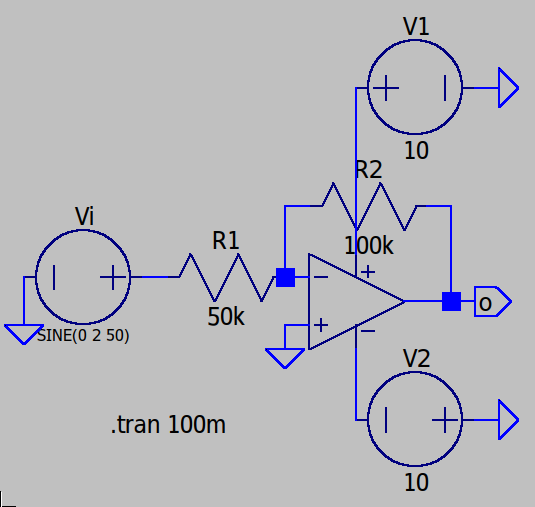
\includegraphics[width=0.36\textwidth]{figures/11c.png} \quad \quad
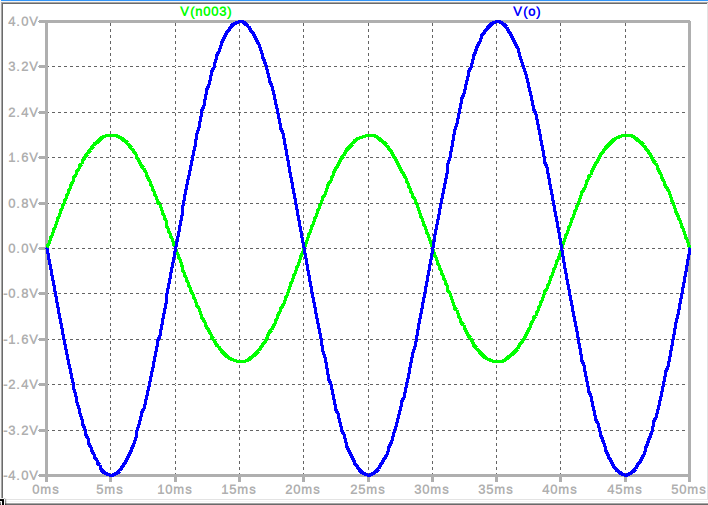
\includegraphics[width=0.47\textwidth]{figures/11w.png} \\
\end{center}
\begin{equation} 
    \notag
    \begin{align*}
    I_\text{R1} = I_\text{R2}\\
    \frac{V_i-0}{R_1} = \frac{0 - V_0}{R_2}\\
    R_2V_i = -R_1V_o\\
    \therefore V_0 = -\frac{R_2}{R_1}V_i
    \end{align}
\end{equation}

\section{Effect of Finite Open-loop Gain}
\begin{equation}
    \notag
    \begin{align*}
    V_o = A(V^+ - V^-)\\
    V^+ = 0 \quad \text{and\ } V^- = -\frac{V_o}{A}\\
    \frac{V_i-(-\frac{V_o}{A})}{R_1} = \frac{-\frac{V_o}{A}-V_o}{R_2}\\
    R_2 V_i + R_2\frac{V_o}{A} = -R_1\frac{V_o}{A} - R_1V_o\\
    R_2 V_i = -V_o(\frac{R_2}{A} + \frac{R_1}{A} + R_1)\\
    \frac{R_2}{R_1}V_i=-V_o(\frac{R_2}{AR_1} + \frac{1}{A} + 1)\\
    \therefore G = \frac{V_o}{V_i} = \frac{-R_2/R_1}{1 + (1 + \frac{R_2}{R_1})/A}
    \end{align*}
\end{equation}
\section{Non-Inverting}
\begin{center}
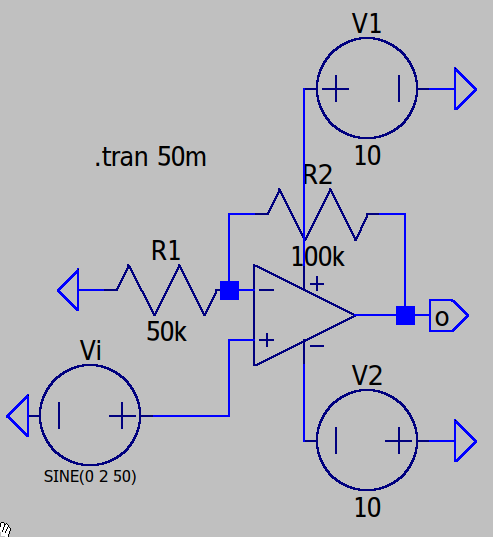
\includegraphics[width=0.35\textwidth]{figures/12c.png} \quad \quad
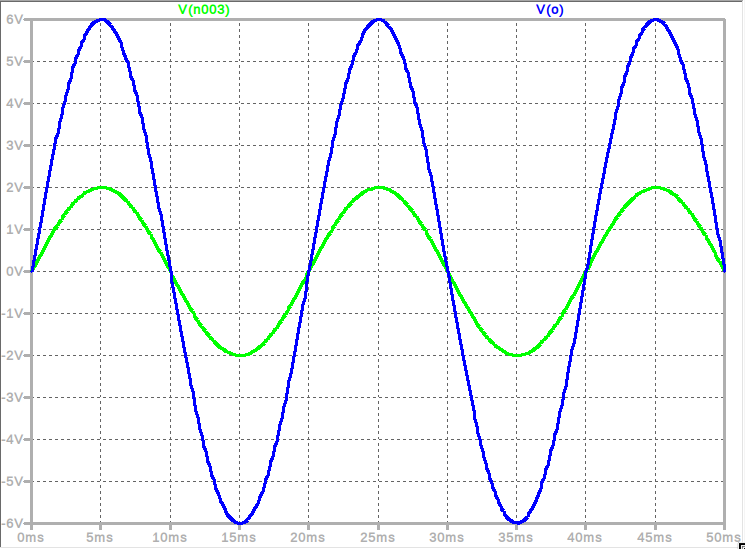
\includegraphics[width=0.5\textwidth]{figures/12w.png} \\
\end{cneter}
\begin{equation}
    \notag
    \begin{align*}
        I_\text{R1} = I_\text{R2}\\
        \frac{0 - V_i}{R_1} = \frac{V_i - V_o}{R_2}\\
        -R_2V_i = R_1V_i-R_1V_o\\
        -V_i(R_2+R_1) = -R_1V_o\\
        \therefore V_o = V_i(1 + R_2/R_1)
    \end{align*}
\end{equation}
\section{Inverting Summer}
\begin{center}
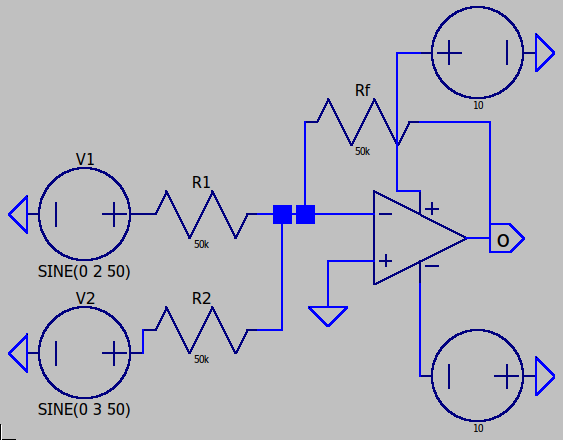
\includegraphics[width=0.4\textwidth]{figures/13c.png} \quad \quad
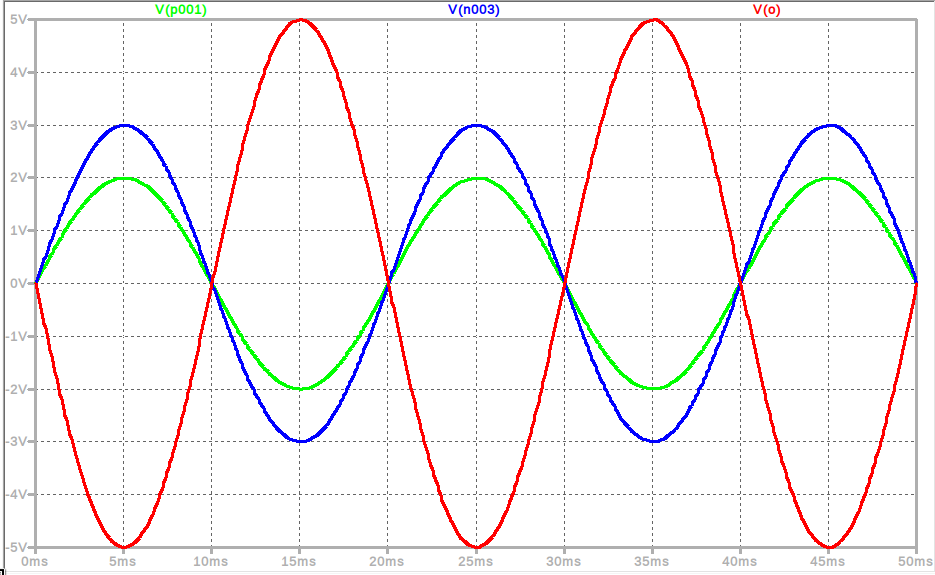
\includegraphics[width=0.5\textwidth]{figures/13w.png} \\
\end{cneter}
\begin{equation}
    \notag
    \begin{align*}
        \because I_\text{R1} + I_\text{R2} = I_\text{$R_f$}\\
        \frac{V_1-0}{R_1} + \frac{V_2-0}{R_2} = \frac{0-V_o}{R_f}\\
        \therefore V_o = -(\frac{R_f}{R_1}V_1 + \frac{R_f}{R_2}V_2)
    \end{align*}
\end{equation}
\section{NonInverting Summer}
\begin{center}
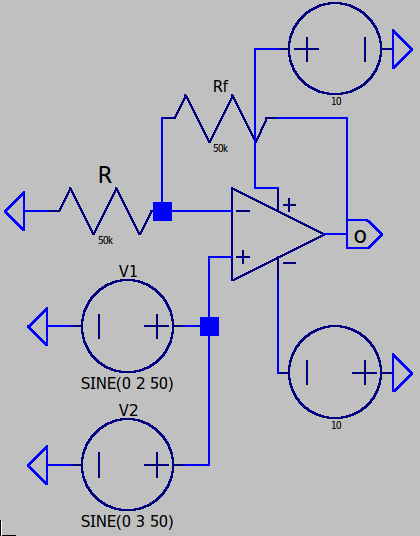
\includegraphics[width=0.3\textwidth]{figures/14c.png} \quad \quad
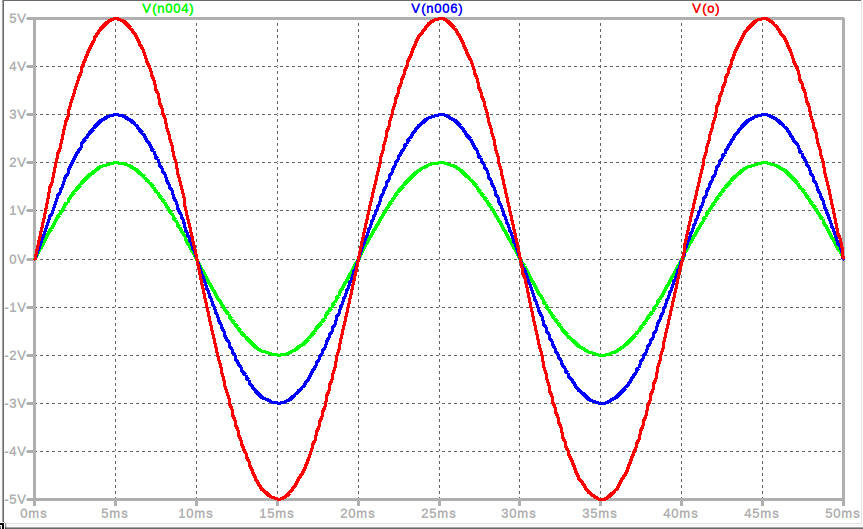
\includegraphics[width=0.56\textwidth]{figures/14w.png} \\
\end{cneter}
\begin{equation}
    \notag
    \begin{align*}
        \because V^- = V^+\\
        \frac{0 - (V_1+V_2)}{R} = \frac{(V_1 + V_2) - V_o}{R_f}\\
        -R_f(V_1+V_2) = R(V_1+V_2) - RV_o\\
        \therefore V_o = (1 + R_f/R)(V_1+V_2)\\
    \end{align*}
\end{equation}

\section{Difference}
\begin{center}
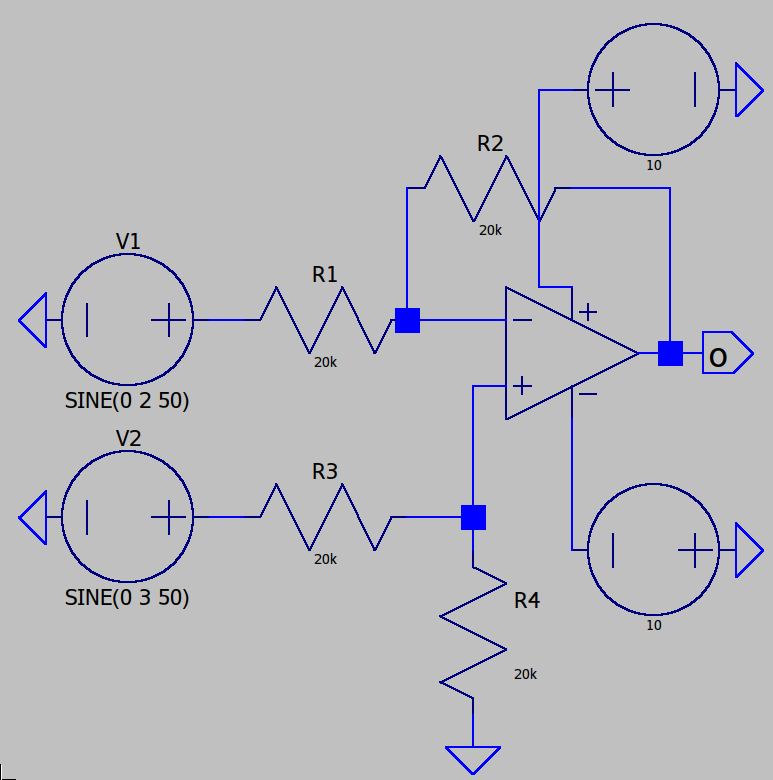
\includegraphics[width=0.4\textwidth]{figures/15c.png} \quad 
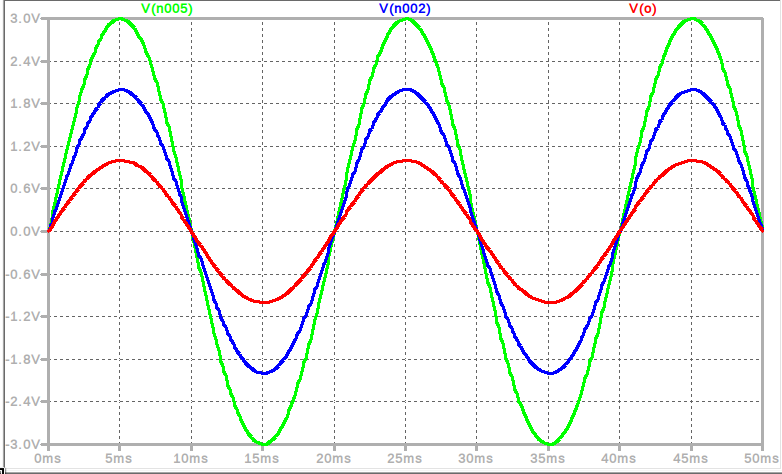
\includegraphics[width=0.55\textwidth]{figures/15w.png} \\
\end{cneter}
\noindent
Using Super position:\\
\begin{equation}
    \notag
    \begin{align}
        \text{kill\ V2:\ }\\
        V_\text{o1} = -\frac{R_2}{R_1}V_1\\
        \text{kill\ V1:\ }\\
        \frac{0 - \frac{R_4}{R_3+R_4}V_2}{R_1} = \frac{\frac{R_4}{R_3+R_4}V_2-V_\text{o2}}{R_2}\\
        \frac{-R_4R_2}{R_3+R_4}V_2 = \frac{R_4R_1}{R_3+R_4}V_2 - R_1V_\text{o2}\\
        V_\text{o2} = \frac{R_2}{R_1}\frac{R_4}{R_3+R_4}V_2 +  \frac{R_4}{R_3+R_4}V_2\\
    \end{align}
        \end{equation}
\begin{equation}
    \notag
    \begin{align}
        V_o = V_\text{o1} + V_\text{o2}\\
        V_o = -\frac{R_2}{R_1}V_1 + \frac{R_2}{R_1}\frac{R_4}{R_3+R_4}V_2 +  \frac{R_4}{R_3+R_4}V_2\\
        V_o = -\frac{R_2}{R_1}V_1 + \frac{R_4}{R_3 + R_4} (\frac{R_2}{R_1}+1)V_2\\
        \text{When\ } R_1 = R_3 \text{,\ } R_2 = R_4\\
        V_o = -\frac{R_2}{R_1}V_1 + \frac{R_2}{R_1 + R_2} (\frac{R_2}{R_1}+1)V_2\\      
        V_o = -\frac{R_2}{R_1}V_1 + \frac{R_2}{R_1 + R_2} (\frac{R_1+R_2}{R_1})V_2\\      
        \therefore V_o = -\frac{R_2}{R_1}(V_2-V_1)      
    \end{align}
\end{equation}
\section{Buffer}
\begin{center}
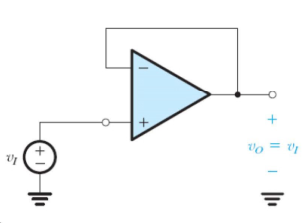
\includegraphics[width=0.45\textwidth]{figures/16c.png}\\ 
\end{cneter}
\begin{equation}
    V_o = V_i 
\end{equation}
\indent
The main function of an op-amp buffer is to provide a high input impedance and a low output impedance, which helps to reduce the loading effect on the circuit it is connected to.
\section{Trans-Impedance}
\begin{center}
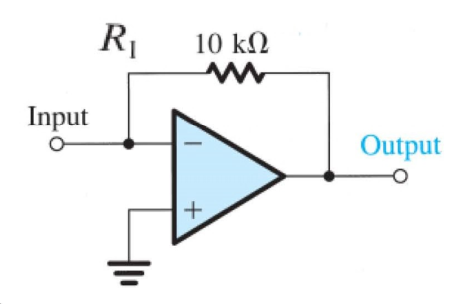
\includegraphics[width=0.45\textwidth]{figures/transimpedance.png} \\
\end{cneter}
\begin{equation}
    \notag
    \begin{align*}
        I_i = I_R\\
        I_i = \frac{0-V_o}{R_f}\\
        \therefore V_o = -R_fI_i
    \end{align*}
\end{equation}
\section{Integrator}
\subsection{Inverting Integrator}
\begin{center}
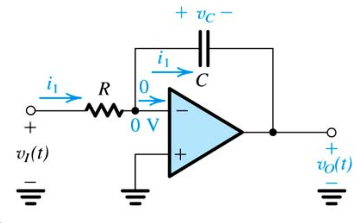
\includegraphics[width=0.4\textwidth]{figures/17c.png}\\ 
\end{cneter}
\begin{equation}
    \notag
    \begin{align*}
        \frac{V_i-0}{R} = I_c\\
        \because V_o = -V_c\\
        \frac{V_i-0}{R} = -C\frac{dV_o}{dt}\\
        \therefore V_o = \frac{-1}{RC}\int V_idt\\
        \text{In\ s\ domain:\ }\\
        V_o = \frac{-1}{sRC}V_i\\
        \frac{V_o(j\omega)}{V_i(j\omega)} = \frac{-1}{(j\omega)RC}\\
        \frac{V_o(j\omega)}{V_i(j\omega)} = \frac{-(-j)}{(\omega)RC}\\
        \text{As\ } j = cos(\frac{\pi}{2}) + jsin(\frac{\pi}{2}) = e^{j\frac{\pi}{2}}\\
        \frac{V_o(\omega)}{V_i(\omega)} = \frac{e^{j\frac{\pi}{2}}}{\omega RC}\\
        \therefore \bigg| \frac{V_o}{V_i}\bigg| = \bigg|\frac{1}{\omega RC}\bigg|\\
 \phi = +90 
    \end{align*}
\end{equation}
\subsection{Miller Integrator}
\begin{center}
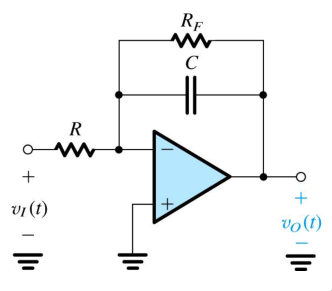
\includegraphics[width=0.37\textwidth]{figures/18c.png} 
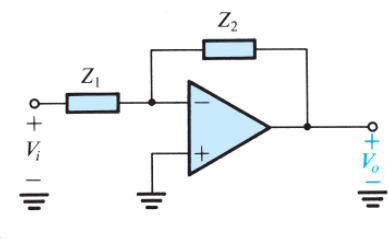
\includegraphics[width=0.38\textwidth]{figures/18w.png}\\ 
\end{cneter}
The Miller integrator with alarge resistance RF connected in parallel with Cin order to provide negative feedback and hence finite gain at dc (A = $\frac{R_f}{R}$).\\
\begin{equation}
    \notag
    \begin{align*}
        V_o = -\frac{Z_2}{Z_1}\\
        Z_2 = \frac{R_f.\frac{1}{sC}}{R_f + \frac{1}{sC}}\\
        Z_2 = \frac{R_f}{sR_fC + 1}\\
        \therefore V_o = \frac{-R_f/R}{sR_fC+1}.V_i\\
    \end{align*}
\end{equation}
\section{Differentiator}
\begin{center}
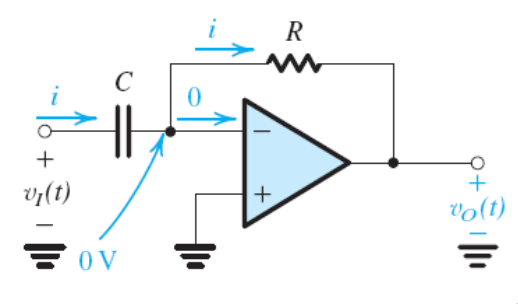
\includegraphics[width=0.4\textwidth]{figures/19c.png} \\
\end{cneter}
\begin{equation}
    \notag
    \begin{align*}
        I_C = I_R\\
        C\frac{dV_i}{dt} = \frac{0-V_o}{R}\\
        \therefore V_o = -RC\frac{dV_i}{dt}\\
    \end{align*}
\end{equation}
\section{Common Mode Gain}
\begin{center}
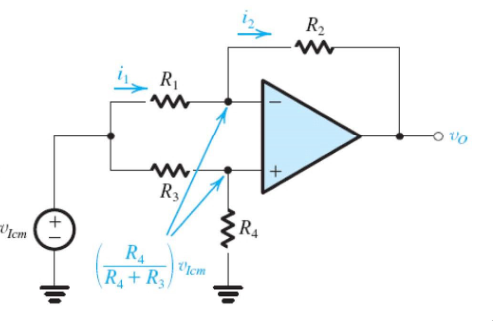
\includegraphics[width=0.45\textwidth]{figures/111c.png} \\
\end{cneter}
\begin{equation}
    \notag
    \begin{align*}
        V^- = \frac{R_4}{R_4 + R_3}V_\text{Icm}\\
        \frac{V_\text{Icm}-V^-}{R_1} = \frac{V_\text{Icm}-V_o}{R_2}\\
        R_2V_\text{Icm} - \frac{R_4R_2}{R_4 + R_3}V_\text{Icm} = \frac{R_4R_1}{R_4 + R_3}V_\text{Icm} - R_1V_o\\
        V_o = \frac{R_2}{R_1}\frac{R_4}{R_4+R_3}V_\text{Icm} + \frac{R_4}{R_4+R_3}V_\text{Icm} - \frac{R_2}{R_1}V_\text{Icm}\\
    \end{align*}
\end{equation}
\begin{equation}
    \notag
    \begin{align*}
        \frac{V_o}{V_\text{Icm}} = \frac{R_4}{R_4+R_3}\bigg(\frac{R_2}{R_1} + 1 - \frac{R_4+R_3}{R_4}.\frac{R_2}{R_1}\bigg)\\
        \frac{V_o}{V_\text{Icm}} = \frac{R_4}{R_4+R_3}\bigg(\frac{R_2}{R_1}(1 - \frac{R_4+R_3}{R_4})+1\bigg)\\
        \frac{V_o}{V_\text{Icm}} = \frac{R_4}{R_4+R_3}\bigg(\frac{R_2}{R_1}(1 - 1 - \frac{R_3}{R_4})+1\bigg)\\
        \therefore A_\text{cm} = \frac{V_o}{V_\text{Icm}} = \frac{R_4}{R_4+R_3}\bigg(1-\frac{R_2}{R_1}\frac{R_3}{R_4}\bigg)\\
    \end{align*}
\end{equation}
When $R_3 = R_1$ and $R_4=R_2$ \\
$A_\text{cm} = 0$
\section{Instrumentation}
To get high input impedance and zero common mode gain (less noise) we can use instrumentation Amplifier.\\
\begin{center}
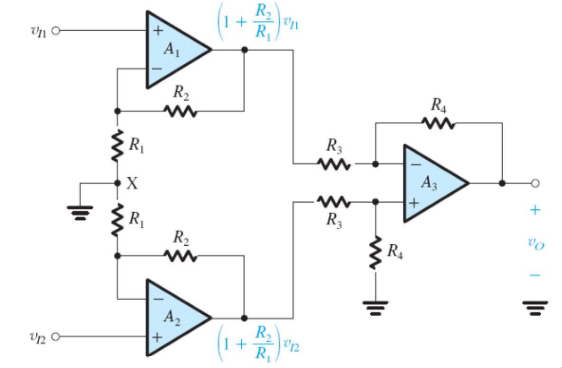
\includegraphics[width=0.5\textwidth]{figures/instrumentation.png} \\
\end{cneter}
\noindent
What're the major disadvantages of this configuration?\\
\indent1- Saturation due to the common mode voltage.\\
\indent2- Common mode voltage will be amplified unless we make perfect matching between\\\indent\indent the resistors which is very hard in practical.\\
\indent3- We have to change at least 2 resistors to change the gain.\\
\begin{center}
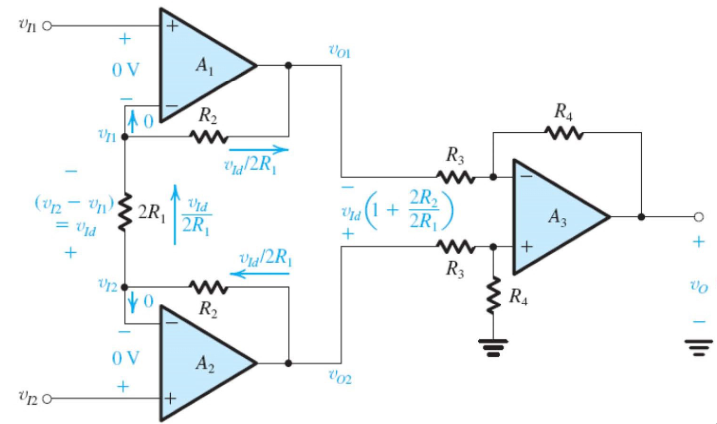
\includegraphics[width=0.5\textwidth]{figures/instrumentation2.png} \\
    \begin{equation}
        \notag
A_\text{cm} = 0\\
A_d = \frac{R_4}{R_3}(1+\frac{2R_2}{2R_1})
    \end{equation}

\end{cneter}

\chapter{Operational Amplifier \\(Non-Linear Applications)}

\section{Comparator}
\subsection{Zero-level detector}
\begin{center}
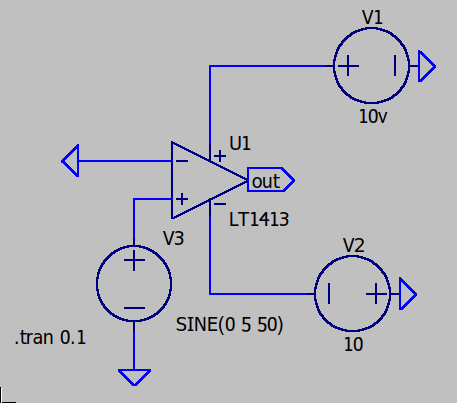
\includegraphics[width=0.32\textwidth]{figures/21c.png} \quad\quad
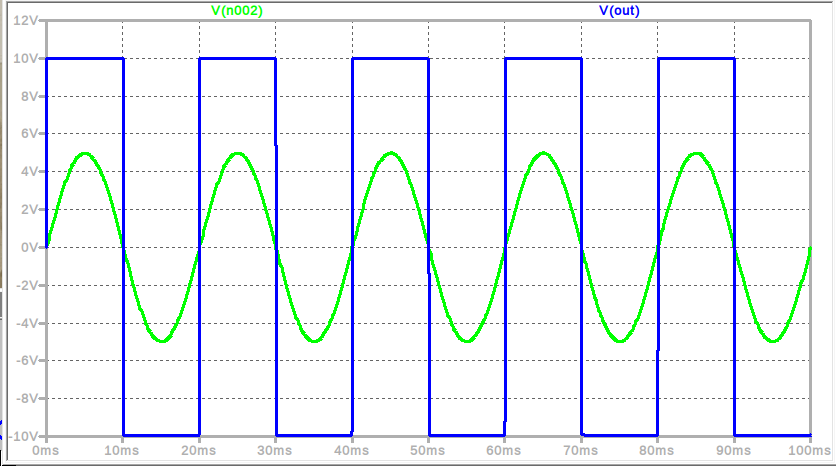
\includegraphics[width=0.5\textwidth]{figures/21w.png} \\
\end{center}
\begin{equation}
    \notag
    \begin{align}
    V_o = A(V^{+} - V^{-}) \\
    \because V^{-} = 0 \\
    V_o = V_\text{cc}
    \end{align}
\end{equation}
\subsection{NonZero-level detector}
\begin{center}
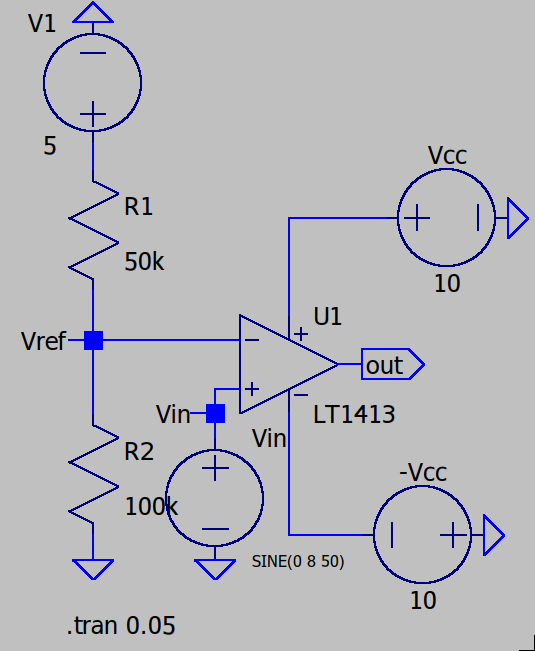
\includegraphics[width=0.25\textwidth]{figures/22c.png}\quad\quad
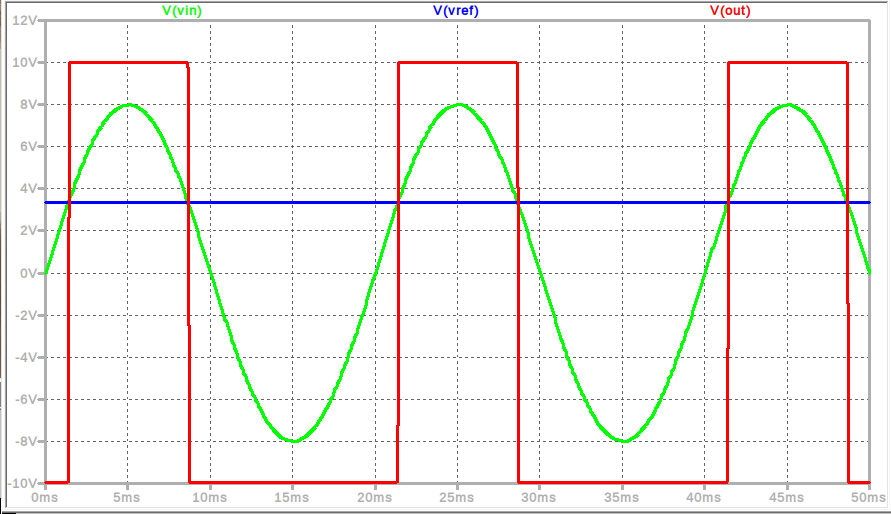
\includegraphics[width=0.53\textwidth]{figures/22w.png}\\
\end{center}
\begin{equation}
    \notag
    \begin{align}
    \because V_o = A(V^{+} - V^{-})\\
    \because V^{-} = V_\text{ref} = V_1 . \frac{R_2}{R_2 + R_1} \\
    \therefore V_o = +V_\text{cc} \quad \text{when} \quad V^{+} > V_\text{ref}\\
    \therefore V_o = -V_\text{cc} \quad \text{when} \quad V^{+} \le V_\text{ref}
    \end{align}
\end{equation}
\subsection{Schmitt Trigger}
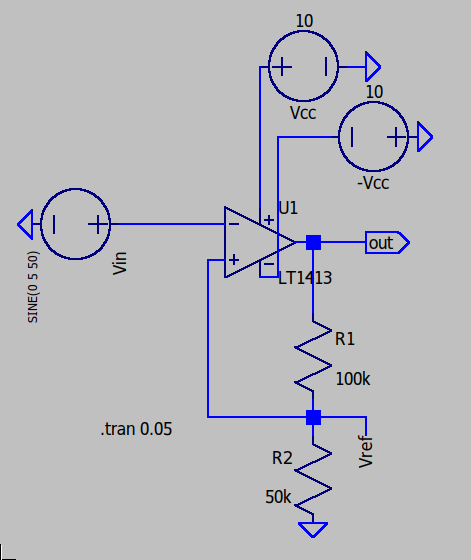
\includegraphics[width=0.32\textwidth]{figures/23c.png}
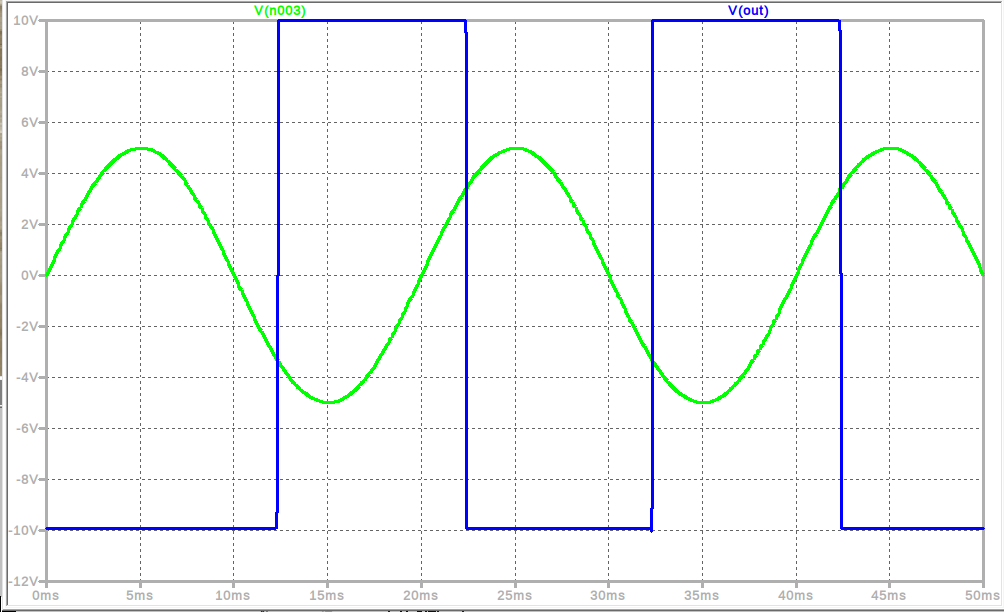
\includegraphics[width=0.45\textwidth]{figures/23w.png}
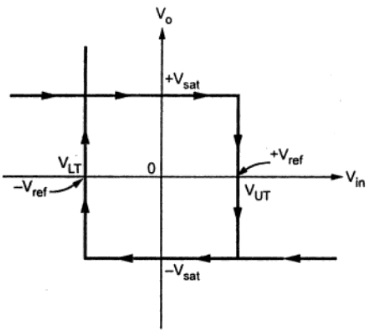
\includegraphics[width=0.33\textwidth]{figures/schmitt.jpg}\\
Using Schmitt Trigger reduces noise effects with hysteresis.

\begin{equation}
    \notag
    \begin{align}
    \because V_o = A(V^{+} - V^{-})\\
    = V_o = A(V_\text{ref} - V_\text{in})\\
    \text{As\ } V_\text{ref} = V_\text{cc} . \frac{R_2}{R_2 + R_1}
    \end{align}
\end{equation}
\section{Practical Triangular-Wave Oscillator}
\begin{center}
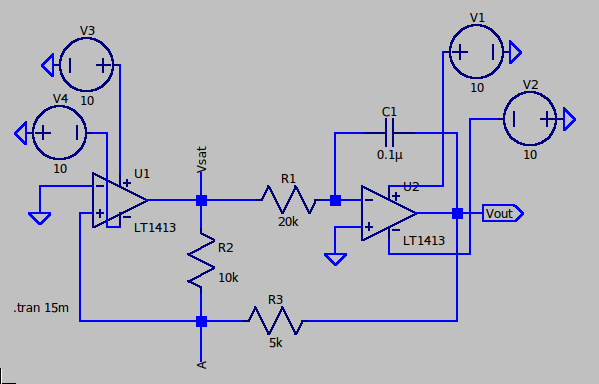
\includegraphics[width=0.48\textwidth]{figures/24c.png}\quad\quad
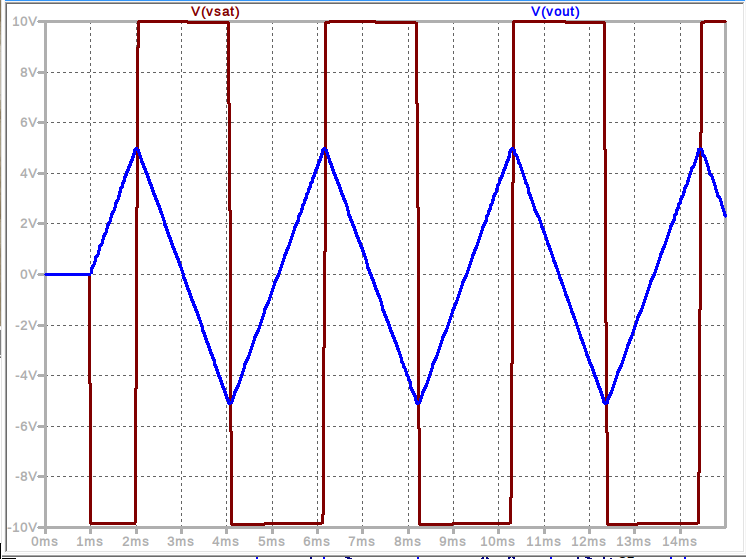
\includegraphics[width=0.41\textwidth]{figures/24w.png}\\
\end{center}
Let $V_\text{UTP}$ be the Upper Trigger Point (UTP) ($V_\text{out}$)\\
And $V_\text{LTP}$ be the Lower Trigger Point (LTP)\\
KCL at pint A:\\
\begin{equation} 
    \notag
    \begin{align*}
    \frac{V_\text{out} - V_A}{R_3} = \frac{V_A - V_\text{sat}}{R_2}\\
        \text{As\ } V_\text{out} = V_\text{UTP} = |V_\text{LTP}|\\
    R_2 V_\text{o} - R_2 V_A = R_3V_A - R_3V_\text{sat}\\
    V_\text{o} = \frac{R_3}{R_2}V_A - \frac{R_3}{R_2}V_\text{sat} + V_A\\
    =\frac{R_3}{R_2}(V_A - V_\text{sat}) + V_A\\
    \text{At\ } V_A = 0\\
    V_\text{o} = -V_\text{sat}\frac{R_3}{R_2}\\
    \end{align*}
\end{equation}
\begin{equation}
    \notag
    \begin{align}
    \text{So\ we\ can\ find\ out\ that:}\\
    V_\text{UTP} = \frac{R_3}{R_2}V_\text{sat}\\
    V_\text{LTP} = -\frac{R_3}{R_2}V_\text{sat}\\
    \end{align}
\end{equation}

4 of the capacitor charging time is the Periodic time.\\
\begin{equation}\notag
    \begin{align}
        V_\text{UTP} = \frac{1}{R_1C} \int dV_\text{sat}dt\\
        \frac{R_3}{R_2}V_\text{sat} = \frac{1}{R_1C} V_\text{sat}t\\
        t = R_1C\frac{R_3}{R_2}\\
        T = 4t = 4\frac{R_3}{R_2}R_1C\\
        \therefore F=\frac{1}{T} = \frac{1}{4R_1C}.\frac{R_2}{R_3}
    \end{align}
\end{equation}
\section{Square-Wave Oscillator (Astable Multivibrator)}
\begin{center}
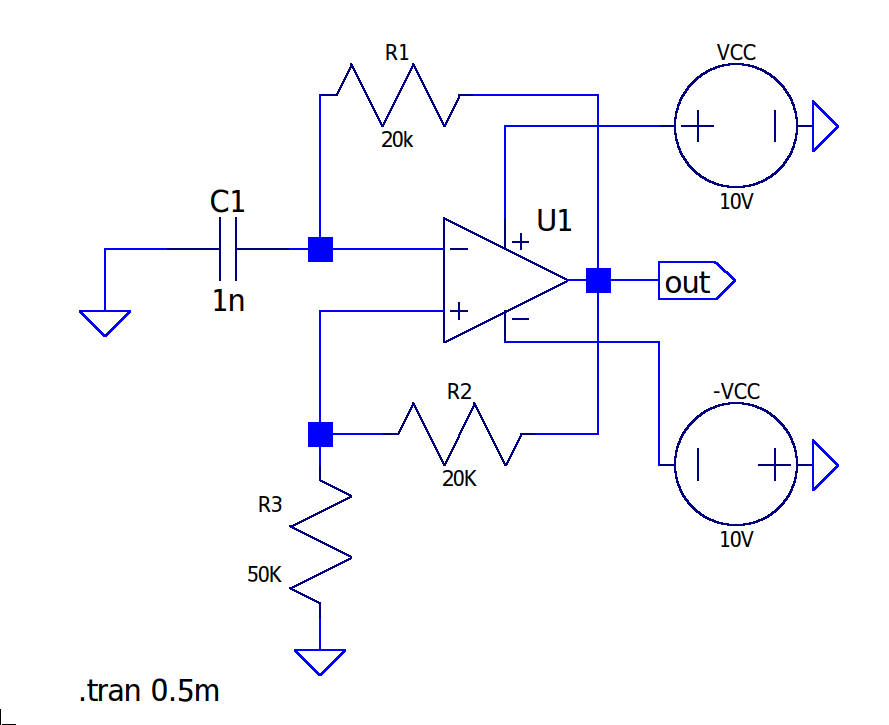
\includegraphics[width=0.4\textwidth]{figures/25c.png}\quad\quad
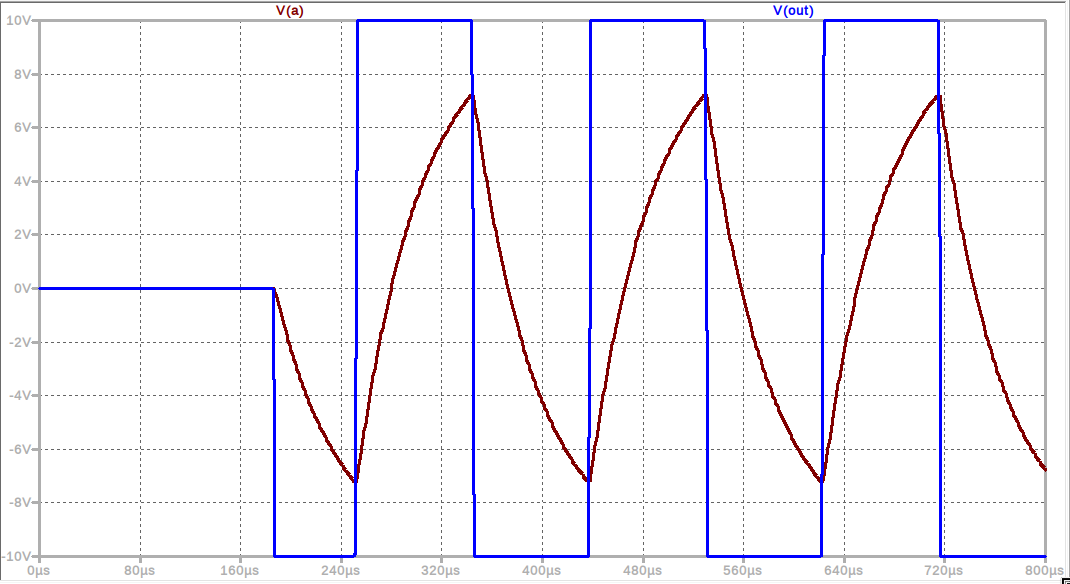
\includegraphics[width=0.49\textwidth]{figures/25w.png}\\
\end{center}
\noindent 
\begin{math}
    \text{When} \quad V_c = 0 \quad \text{and\ Capacitor\ begins\ charging}\\
    \because V_o = A\cdot(V_f - V_c) \\
    \because V_f > V_c\\
    \therefore V_o = V_\text{sat} \\
    \text{When\ } V_c \ge V_f \\
    V_o = - V_\text{sat}\\
    \because V_f = \beta V_\text{sat} \quad \text{As\ } \beta = \frac{R_3}{R_3+R_2} \\
    \text{Using\ KCL\ }
\end{math}
\begin{equation}
    \notag
    \frac{V_\text{sat} - V_c}{R_1} = C\frac{dV_c}{dt}\\
\end{equation}

\begin{equation}
    \notag
    \frac{V_\text{sat} - V_c}{R_1C} = \frac{dV_c}{dt}\\
\end{equation}

\begin{equation}    \notag
    \int_{0}^{t}  \frac{dt}{R_1C} = \int_{-v_f}^{v_f} \frac{dV_c}{V_\text{sat} - V_c}
\end{equation}

\begin{equation}    \notag
    \frac{t}{R_1C} = \ln (V_\text{sat} + V_f) - \ln (V_\text{sat} - V_f)
\end{equation}

\begin{equation}    \notag
    \frac{t}{R_1C} = \ln (\frac{V_\text{sat} + V_f}{V_\text{sat}-V_f})   
\end{equation}

\begin{equation}    \notag
    t = R_1C . \ln (\frac{1 + \beta}{1-\beta})   
\end{equation}

\begin{equation}    \notag
    T = 2t = 2R_1C . \ln (\frac{1 + \beta}{1-\beta})   
\end{equation}

\begin{equation}    \notag
    \therefore F = \frac{1}{2R_1C . \ln (\dfrac{1 + \beta}{1-\beta})}   
\end{equation}

\section{Log and Antilog Amplifier}
\begin{multicols}{2}
\subsection{Basic log Amplifier}
\begin{center}
    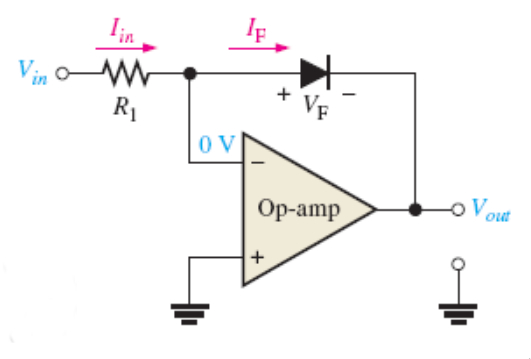
\includegraphics[width=0.44\textwidth]{figures/26c.jpg}
\end{center}
\begin{equation} \notag
    \begin{align}
    I_D = I_F = I_R e^\frac{V_F}{V_T}\\
    I_R \quad \text{is\ const\ }\\
    V_T = \frac{q}{kt} \approx 26mV\\
    V_o = -V_F\\
    \text{Using\ KCL:\ }\\
    I_\text{in} = I_F\\
    \frac{V\text{in}}{R_1} = I_R e^{\frac{-V_o}{V_T}}\\
    \frac{-V_o}{V_T} = \ln(\frac{V_\text{in}}{R_1I_R})\\
    \therefore V_o = -V_T \ln(\frac{V_\text{in}}{R_1I_R})
    \end{align}
\end{equation}

\subsection{Log Amplifier with BJT}
\begin{center}
    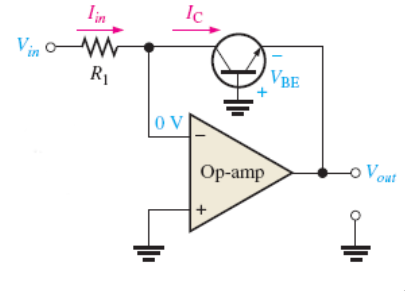
\includegraphics[width=0.41\textwidth]{figures/27c.png}
\end{center}
\begin{equation} \notag
    \begin{align}
        I_E = I_C + I_B\\
        I_C >> I_B\\
        I_E \approx I_C\\
        I_c  = I_\text{EBO} e^{\frac{V_\text{BE}}{V_T}}\\
        I_\text{in} = I_C\\
        \frac{V_i}{R_1} = I_\text{EBO}e^{\frac{-V_o}{V_T}}\\
    \therefore V_o = -V_T \ln(\frac{V_\text{in}}{R_1I_\text{EBO}})
    \end{align}
\end{equation}
\end{multicols}
\subsection{Basic Antilog}
\begin{multicols}{2}
    \begin{equation}\notag
        \begin{align}
            V_o = -R_fI_C \\
            I_C = I_\text{EBO}e^{\frac{V_i}{V_T}}\\
            \therefore V_o = -R_fI_\text{EBO}e^{\frac{V_i}{V_T}}\\
            V_o = -R_f I_\text{EBO} \text{antilog}(\frac{V_i}{26mV})
        \end{align}
    \end{equation}
\begin{center}
    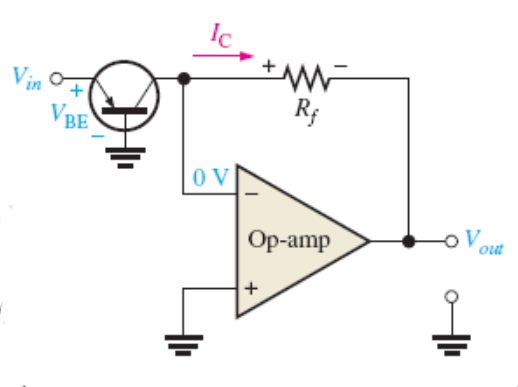
\includegraphics[width=0.37\textwidth]{figures/28c.png}
\end{center}
\end{multicols}

\begin{multicols}{2}
\section{Multiplier}
\begin{center}
    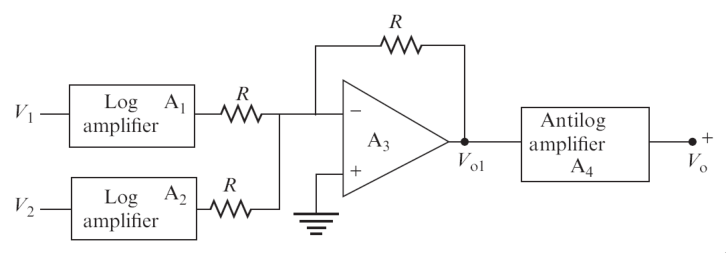
\includegraphics[width=0.55\textwidth]{figures/29c.png}
\end{center}
\begin{equation} \notag
    \begin{align}
        V_\text{o1} = V_T\bigg(ln(\frac{V_1}{RI_\text{EBO}}) + ln(\frac{V_2}{RI_\text{EBO}})\bigg)\\
        = V_T\bigg(ln(\frac{V_1V_2}{R^2I^2_\text{EBO}})\bigg)\\
        V_o = -R I_\text{EBO} e^{ln(\frac{V_1V_2}{R^2I^2_\text{EBO}})}\\
        = -R I_\text{EBO} \frac{V_1V_2}{R^2I^2_\text{EBO}}\\
        \therefore V_o = - \frac{V_1V_2}{RI_\text{EBO}}\\
    \end{align}
\end{equation}

\section{Divider}
\begin{center}
    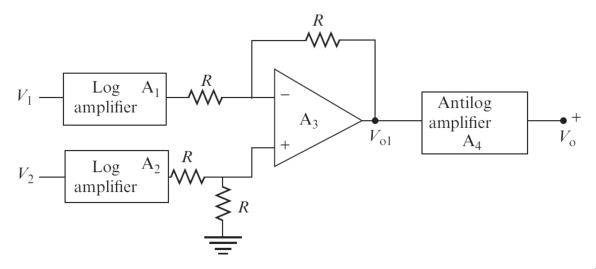
\includegraphics[width=0.55\textwidth]{figures/210c.png}
\end{center}
\begin{equation} \notag
    \begin{align}
        V_\text{o1} = -V_T ln\big(\frac{V_2}{RI_\text{EBO}}\big) + V_T ln\big(\frac{V_1}{RI_\text{EBO}}\big)\\
        = V_T\bigg(ln(\frac{V_1}{V_2})\bigg)\\
        V_o = -RI_\text{EBO}e^{ln(\frac{V_1}{V_2})}\\
        \therefore V_o = -RI_\text{EBO} \frac{V_1}{V_2}
        \\
        \\
    \end{align}
\end{equation}
\end{multicols}
\section{Positive half-wave rectifier}
\begin{center}
    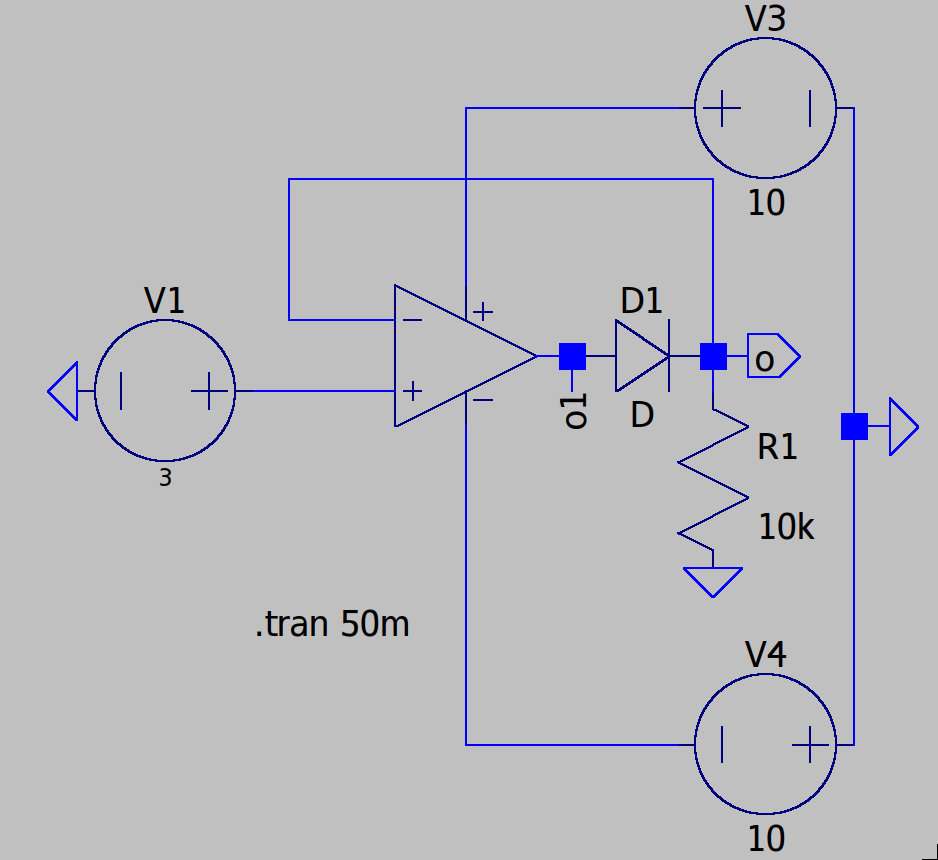
\includegraphics[width=0.35\textwidth]{figures/211c.png}\quad\quad
    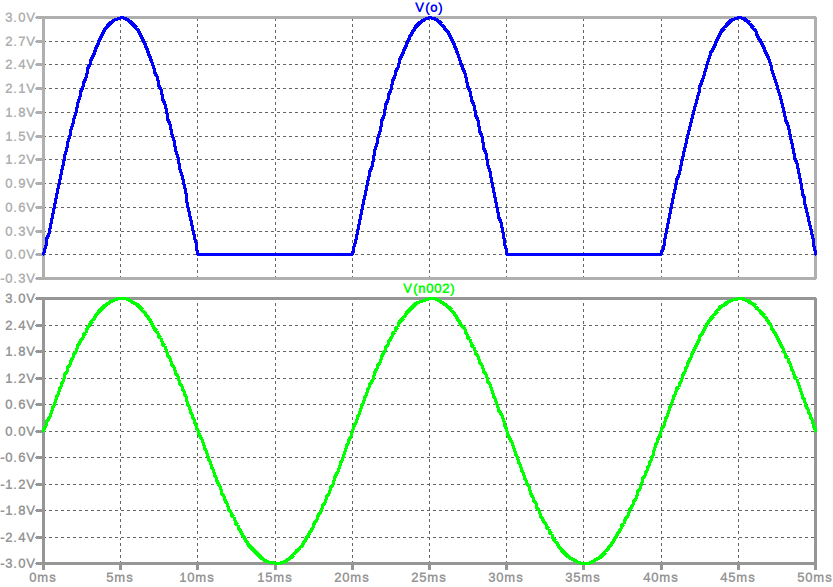
\includegraphics[width=0.45\textwidth]{figures/211w.png}\\
\end{center}
\begin{equation}
\notag
    \begin{align}
        V_\text{o1} \approx V_1 + 0.623\\
        V_o = V_1 \text{\ Rectified}
    \end{align}
\end{equation}
\pagebreak
\section{Full-wave Rectifier}
\begin{center}
    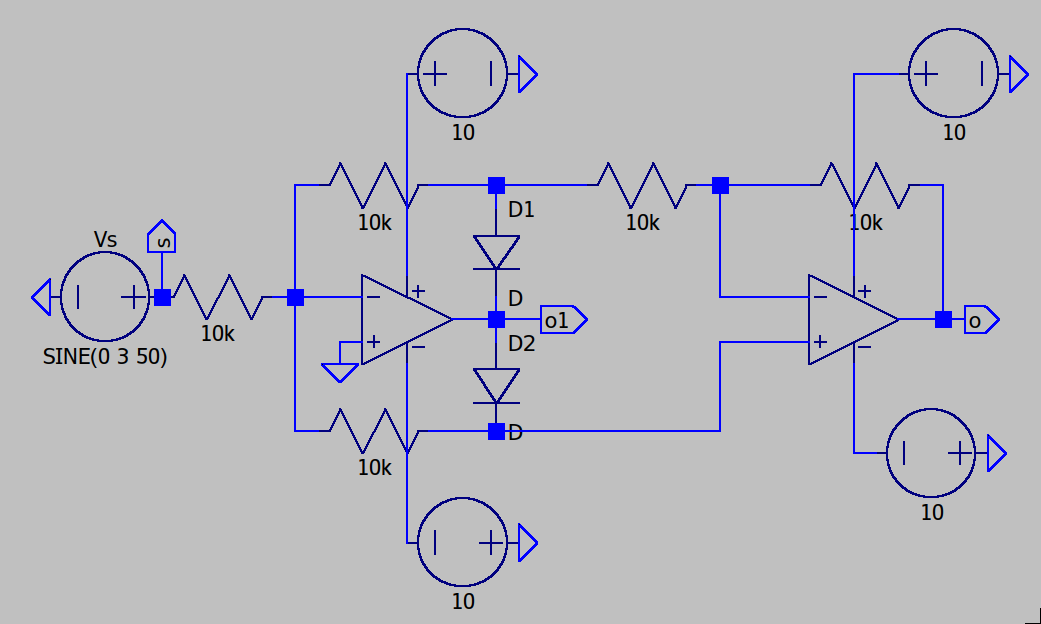
\includegraphics[width=0.52\textwidth]{figures/212c.png}\quad
    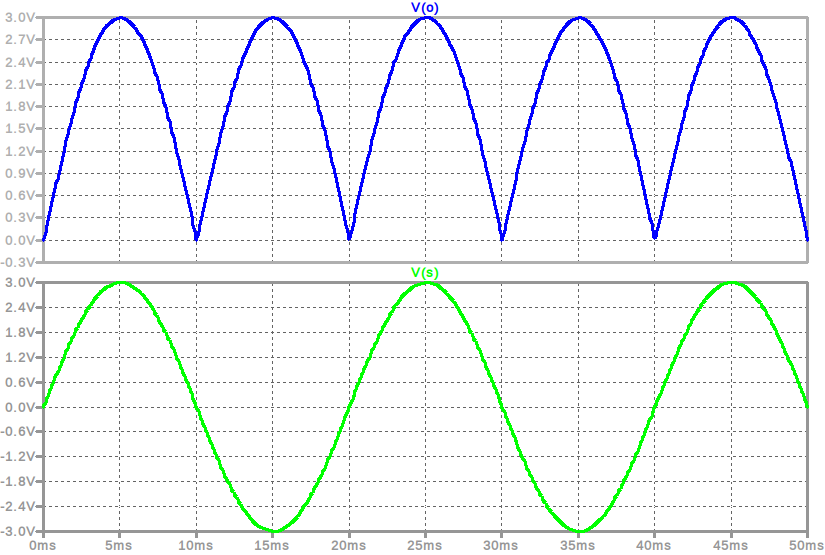
\includegraphics[width=0.45\textwidth]{figures/212w.png}\\
\end{center}

\begin{multicols}{2}
    \subsection*{During positive half cycle}
    \begin{center}
        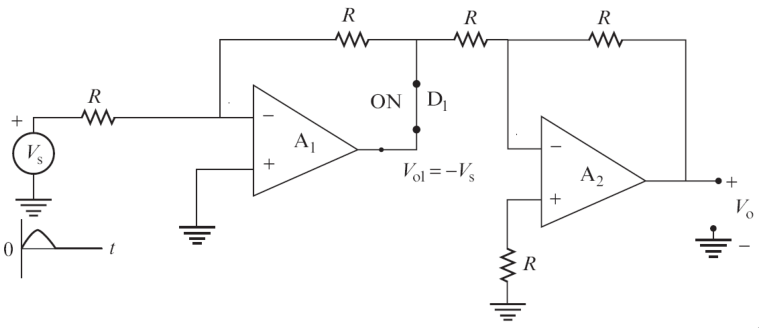
\includegraphics[width=0.55\textwidth]{figures/212c2.png}\\
    \end{center}
    \begin{equation}\notag
        \begin{align}
            \frac{V_s-o}{R} = \frac{0-V_\text{o1}}{R}\\
            V_\text{o1} = -V_s\\
            \frac{V_\text{o1}-o}{R} = \frac{0-V_o}{R}\\
            V_o = -V_\text{o1}\\
            \therefore V_o = V_s\\
            \\
            \\
            \\
            \\
        \end{align}
    \end{equation}

    \subsection*{During negative half cycle}
    \begin{center}
        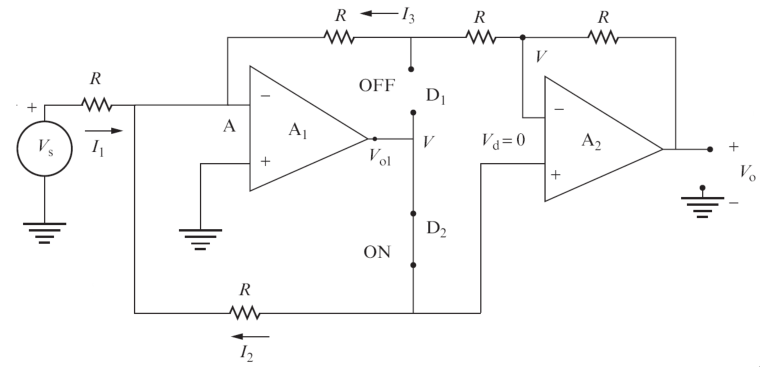
\includegraphics[width=0.5\textwidth]{figures/212c1.png}\\
    \end{center}
    \begin{equation}\notag
        \begin{align}
            I_1 + I_2 + I_3 = 0\\
            \frac{V_s}{R} + \frac{V}{R} + \frac{V}{2R} = 0\\
            V = -\frac{2}{3}V_s\\
            \frac{0-V}{2R} = \frac{V-V_o}{R}\\
            V_o = \frac{3}{2}V\\
            V_o = \frac{3}{2}\bigg(-\frac{2}{3}V_s\bigg)\\
            \therefore V_o = -V_s
        \end{align}
    \end{equation}
\end{multicols}
\chapter{Timer 555}
\section{Monostable Multivibrator}
\begin{center}
    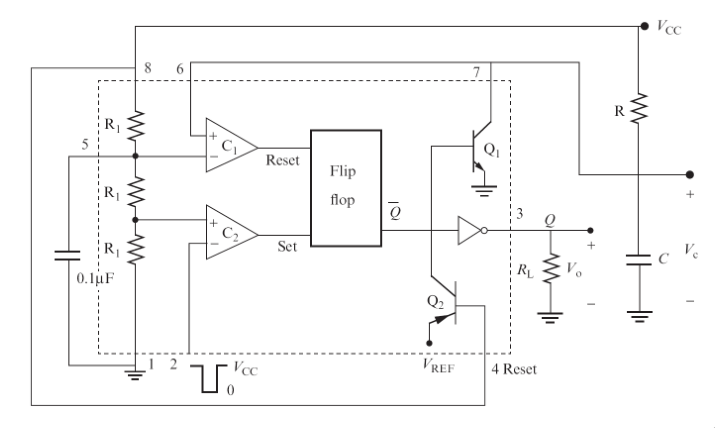
\includegraphics[width=0.65\textwidth]{figures/timermono.png}
\end{center}
\begin{center}
    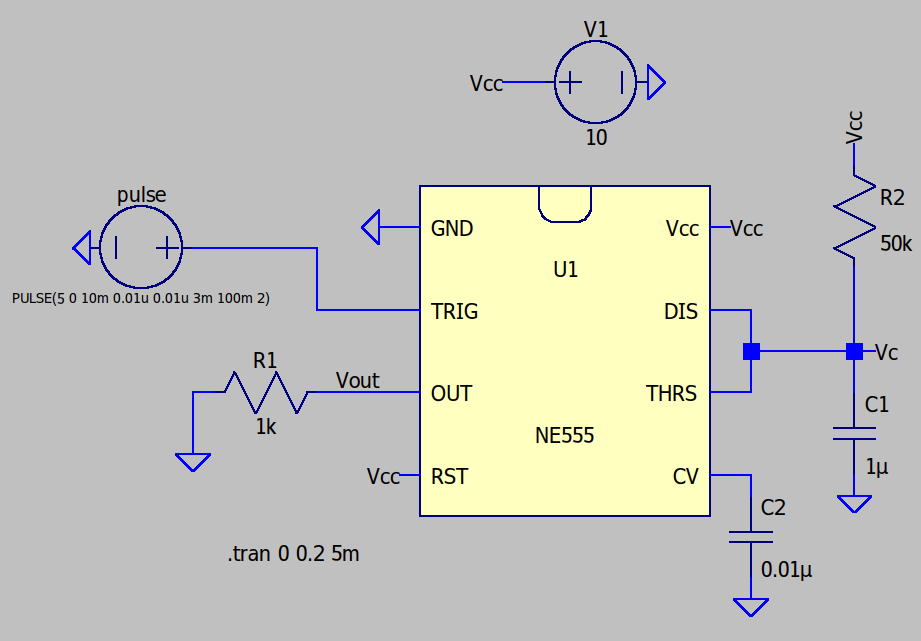
\includegraphics[width=0.45\textwidth]{figures/31c.png}
    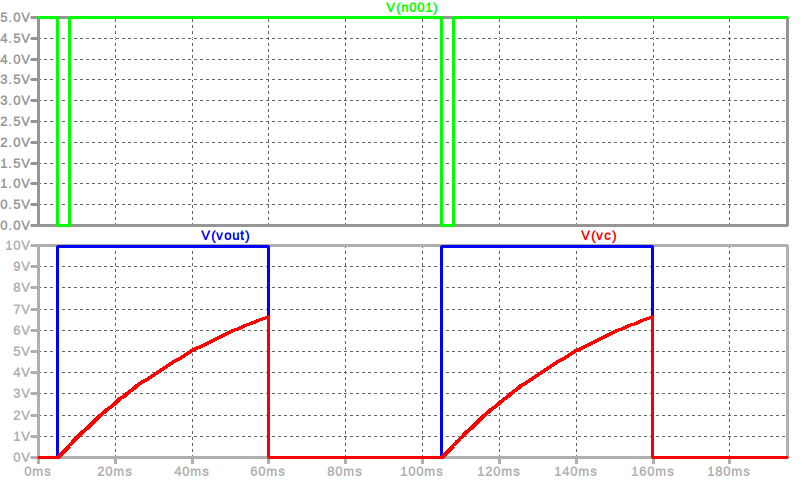
\includegraphics[width=0.52\textwidth]{figures/31w.png}\\
\end{center}
\begin{equation}\notag
        \begin{align}
            V_c(t) = V_F - (V_F - V_I)e^{\frac{-t}{\tau}}\\
            V_c(t) = V_\text{cc} - (V_\text{cc} - o)e^{\frac{-t}{RC}}\\
            \text{At\ } t = T \text{,\ } V_c(t) = \frac{2}{3}V_\text{cc}\\
            \frac{2}{3}V_\text{cc} = V_\text{cc}\bigg(1-e^{\frac{-T}{RC}}\bigg)\\
            e^{\frac{-T}{RC}} = \frac{1}{3}\\
            \frac{-T}{RC} \approx -1.1\\
            \therefore T = 1.1RC
        \end{align}
    \end{equation}
\section{Astable Multivibrator}

\end{document}
